\subsubsection{Newton's Method}
Another approach is called Newton's method, which is also rooted in the Taylor approximation. However, this method also uses the second order term of the approximation.\cite{AAntoniou}
%
\begin{flalign}
  f(\vec{x}+\vec{\delta}) &\approx f(\vec{x}) + \vec{g}^T \vec{\delta} + \frac{1}{2} \vec{\delta}^T \vec{H}\vec{\delta} &
\label{taylorApproximation2ndOrder}
\end{flalign}

In this case the derivative of the approximation is set to 0, and the following is obtained.\cite{AAntoniou}
%
\begin{flalign}
  \nabla\ f(\vec{x}+\vec{\delta}) &\approx \vec{g} + \frac{1}{2}\ \nabla\ \vec{H}\vec{\delta}^2 &\\
  \nabla f(\vec{x}+\vec{\delta}) &\approx \vec{g} + \vec{H}\vec{\delta} = 0 &
\label{2stOrderTaylorApproximationParThetaEqZero}
\end{flalign}

Using this to find an expression for the difference in \si{\vec{x}}, \si{\vec{\delta}}, yields the following.\cite{AAntoniou}
%
\begin{flalign}
  0 &= \vec{g} + \vec{H}\vec{\delta}  &\\
  \vec{\delta} &= -\vec{H}^{-1}\vec{g} &
\label{NewtonsMethod}
\end{flalign}

%This expression can then be used to choose the value of \si{\vec{\delta}} such that the approximation of \si{f(\vec{x})} is minimized. An implementation where it is possible to directly retrieve the gradient and a Hessian of the function which is to be minimized, \si{f(\vec{x})}, is shown in \figref{NewtonsMethodEx}. 
%%
%\begin{figure}[H] 
%	\centering
%	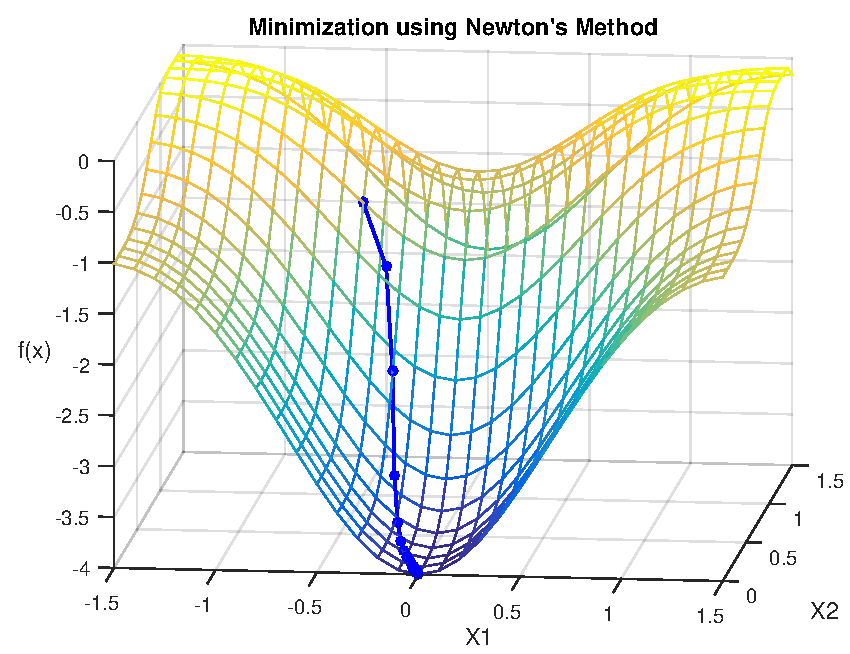
\includegraphics[width=.7\textwidth]{figures/NewtonsMethodEx}
%	\caption{Example of a direct implementation of Newton's method for optimization.}
%	\label{NewtonsMethodEx}
%\end{figure}
%
%If compared to the steepest descend method in \figref{steepestDescendEx} and \ref{steepestDesendExZoom}, where 100 iterations were used, it is clear how Newton's method converges much faster, in 30 iterations, to the minimum of \si{f(\vec{x})}. 

The gradient is found in the previous section, the Hessian is also needed and can be related to to gradient as follows.\cite{Senstools}
%
\begin{flalign}
	\vec{H}(\vec{\theta}) &= \nabla\ (\nabla\  P(\vec{\theta})) = \nabla\ \vec{G}(\vec{\theta}) &
\end{flalign}
%
%which leads to the following:
%\begin{flalign}
%	\vec{H}(\vec{\theta}) &= \frac{1}{N}\sum_{k = 1}^{N} \left(\nabla \ \vec{y_m}(kT, \vec{\theta}) \left(\nabla \ \vec{y_m}(kT, \vec{\theta}) \right)^T  	  - \left(\nabla\ (\nabla\ \vec{y_m}(kT, \vec{\theta})) \right) (\vec{y}(kT) - \vec{y_m}(kT, \vec{\theta}))  \right) &
%\label{hessianOfPerformanceFunction}
%\end{flalign}

To avoid the second derivative of the performance function in \eqref{hessianOfPerformanceFunction}, the Hessian can be approximated simply by removing the 2nd derivative therm, which leads to the following.\cite{Senstools}
\begin{flalign}
	\vec{\widetilde{H}}(\vec{\theta}) &\triangleq \frac{1}{N} (\nabla \ \vec{y_m} (\vec{\theta})) \left(\nabla \ \vec{y_m}(\vec{\theta}) \right)^T &
\label{hessianApproxOfPerformanceFunction}
\end{flalign}

This approximation assumes that the model is only linearly dependent on the parameters, \si{\vec{\theta}}. As the error term, \si{(\vec{y} - \vec{y_m}(\vec{\theta}))}, approaches zero the approximation becomes increasingly accurate.